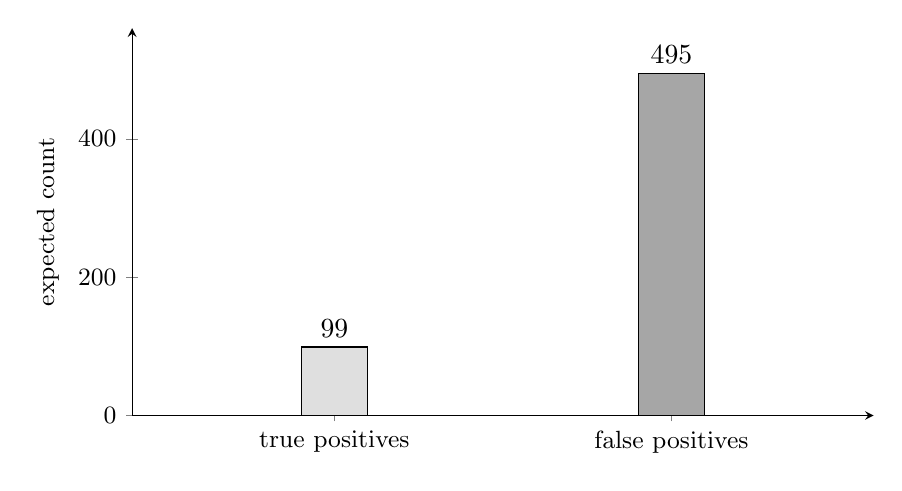
\begin{tikzpicture}
\begin{axis}[width=11cm,height=6.5cm,axis lines=left,tick label style={font=\small},label style={font=\small},legend style={font=\scriptsize},xtick={1,2},xticklabels={true positives,false positives},ylabel={expected count},xmin=0.4,xmax=2.6,ymin=0,ymax=560]
\addplot[ybar,bar width=24pt,fill=gray!25,draw=black] coordinates {(1,99)};
\addplot[ybar,bar width=24pt,fill=gray!70,draw=black] coordinates {(2,495)};
\node[above] at (axis cs:1,99) {$99$};\node[above] at (axis cs:2,495) {$495$};
\end{axis}\end{tikzpicture}
